%\chapter{Génération des harnais de tests, Model testing}
\chapter{Test du modèle et génération du harnais}
\label{chap:harnais}

Ce chapitre est basé principalement sur les recherches précédentes des étudiants de Master 1 et de Master 2 dont nous avons utilisé les rapports pour avancer dans notre travail.

Notre objectif étant d'effectuer une comparaison entre le test du modèle et le test du code, comme le travail sur le test du code avait déjà été effectué en amont par le groupe d'étudiants de Master 2\cite{rapportM2}, nous nous sommes documentés sur cette étape sans y apporter de nouvelles informations. 

Ce chapitre repose principalement sur les rapports des étudiants précédents et sur la documentation disponible sur le site de COSTO\footnote{\url{http://costo.univ-nantes.fr/}}. Nous avons choisi de reprendre ces informations parce que nous avons passé du temps à les comprendre et qu'il nous parait important d'avoir une explication du modèle et de la génération du harnais au sein de ce rapport.



\section{Modèle utilisé : Platoon System}
\label{sec:harnaisModele}

Pour le test du modèle et la génération du harnais, nous avons travaillé avec l'exemple du PlatoonSystem\footnote{\url{http://costo.univ-nantes.fr/application/vehicle-exemple/}} qui est un modèle représentant un système de véhicules qui se suivent avec un pilote au départ. Ce modèle est représenté schématiquement par la figure \ref{fig:platoonSchema} avec les services fournis et requis. Ces véhicules doivent répondre à des contraintes de vitesse minimale, maximale et de distance de sécurité, chaque véhicule modifiant sa vitesse en fonction de celle du véhicule devant lui.

\begin{figure}[H]
    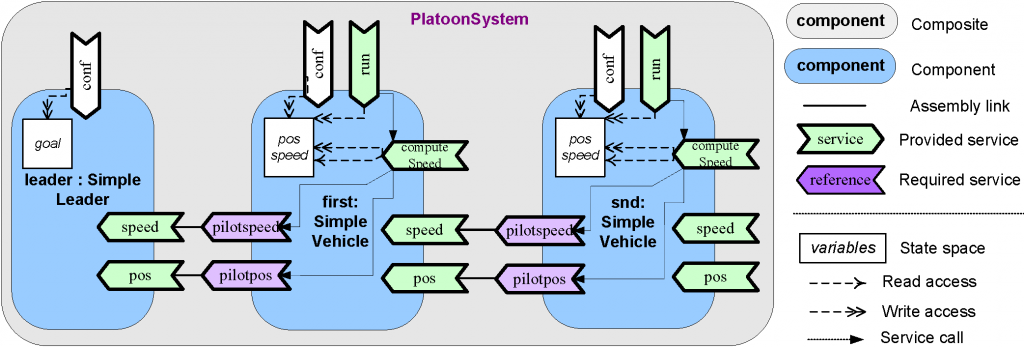
\includegraphics[scale=0.35]{images/platoonSchema.png}
    \caption{Schéma du PlatoonSystem}
    \label{fig:platoonSchema}
\end{figure}


\section{Génération du harnais de test}
\label{sec:harnaisGeneration}

COSTOTest est le plugin servant à générer et lancer les harnais de tests, on l'utilise en lançant Eclipse avec la bonne installation\footnote{\url{http://costo.univ-nantes.fr/tools/technical-environment-of-costo/eclipse-installation/}}

Pour lancer le harnais il faut cliquer sur \textit{GenerateTH}, ensuite il faut sélectionner le service à tester. Ensuite le plugin affiche une fenêtre où il est possible de placer des mocks sur les services nécessaires au test. Une fois que tout est paramétré, il est possible de lancer le harnais de test. Une fenêtre s'ouvre et permet de choisir quelle valeur les mocks doivent renvoyer, le harnais procède à un test sur ces valeurs et génère un fichier de verdict. Par la suite il est possible de réutiliser un harnais de test sans devoir le re-paramétrer si on souhaite faire un test sur des valeurs. Il est aussi possible de tester plusieurs jeux de valeurs en même temps il suffit de préciser le nombre que l'on souhaite et de fournir les données de tests.
\clearpage
    \topskip0pt
    \vspace*{\fill}
\begin{figure}[H]
    \begin{center}
        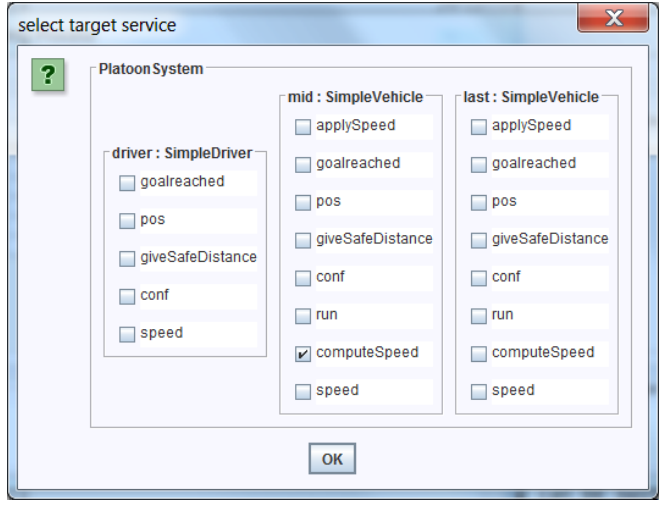
\includegraphics[scale=0.8]{images/SelectionServiceCOSTOTest.png}
        \caption{Image sélection de service COSTOTest}
        \label{fig:SelectionServiceCOSTOTest}
    \end{center}
\end{figure}

    \vspace*{\fill}
    \clearpage
    \topskip0pt
    \vspace*{\fill}
 
 Voici l'écran sur lequel on peut rentrer les valeurs de test et où on peut créer des mocks. 
\begin{figure}[H]
    \begin{center}
        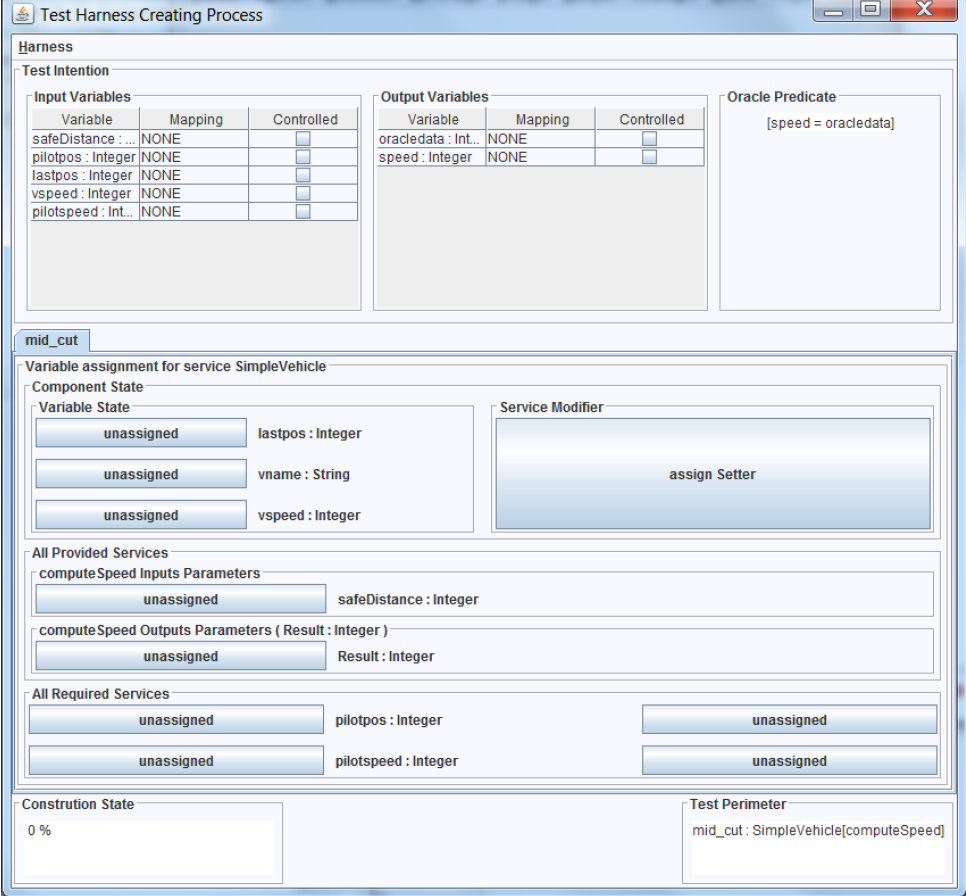
\includegraphics[scale=0.6]{images/CreationMockCOSTOTest.png}
        \caption{Image sélection des valeur du test et crétion des mocks COSTOTest}
        \label{fig:CreationMockCOSTOTest}
    \end{center}
\end{figure}

    \vspace*{\fill}
    \clearpage
    \topskip0pt
    \vspace*{\fill}

Et voici à quoi ressemble un harnais de test complété sur le service \textit{computeSpeed}
\begin{figure}[H]
    \begin{center}
        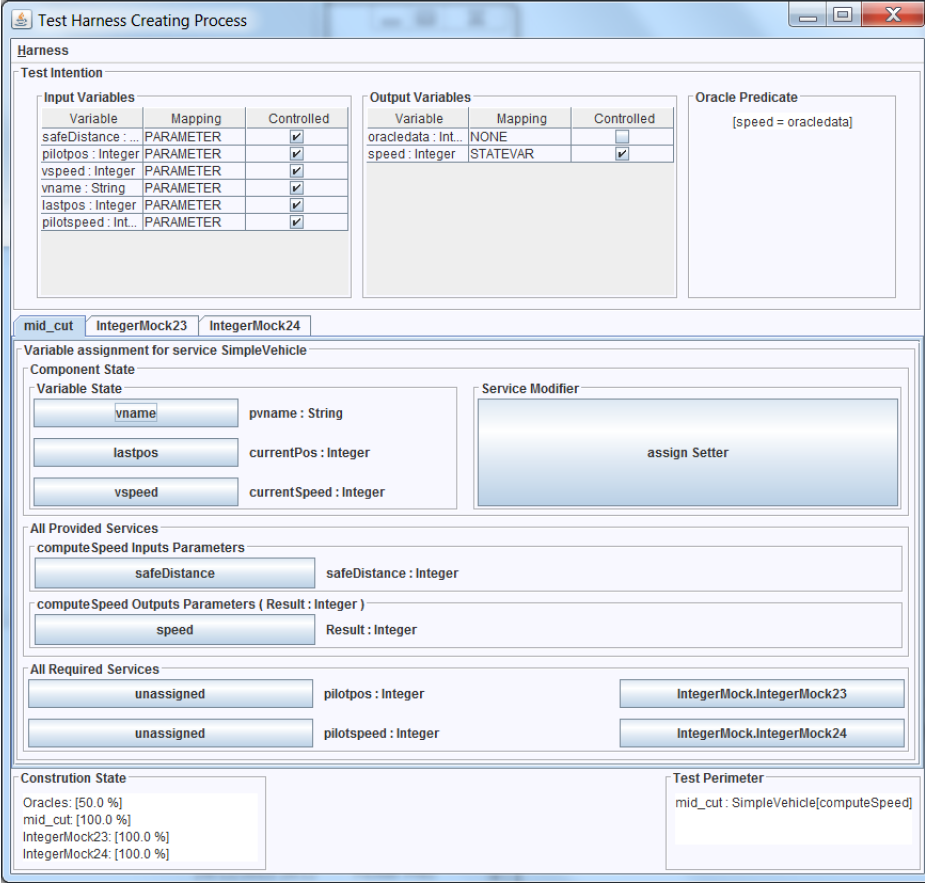
\includegraphics[scale=0.55]{images/HarnaisFiniCOSTOTest.png}
        \caption{Harnais complété COSTOTest}
        \label{fig:SelectionServiceCOSTOTest}
    \end{center}
\end{figure}

    \vspace*{\fill}

